\chapter{Projekte}\index{chp\_Projekte}

\section{Systemrecorder}
\subsection{Aufgabenstellung}
Erarbeitung einer Möglichkeit die Daten nativ auf dem Linux Gerät, als auch im Webbrowser graphisch aufzubereiten, wobei die Konformität an Stilrichtlinien gegeben sein muss.
Des Weiteren sollte erreicht werden, dass es nur noch eine Codebase gibt. 
\subsection{Bisheriger Stand}
In den Geräten der W (für Wireless) und M (für Mobile) aus der SCALANCE Produktlinie gibt es aktuell eine Schnittstelle in der im WBM (engl. für Web Based Management) wichtige Kenndaten zur Signalqualität des Wireless Lan bzw. Mobilfunk(LTE - Long Term Evolution bzw. 4G sowie 5G) Signals grafisch aufbereitet werden. \\
Dies dient zum einen zur generellen Einschätzung der aktuellen Signalparameter sowie zur Vereinfachung von Problemen im Netzwerk beziehungsweise in der Verbindung. Diese generierten Daten 
können einerseits über eine auf dem Gerät generierte PDF beziehungsweise CSV Datei weitergegeben werden als auch direkt im WBM zum aktuellen Zeitpunkt angezeigt werden. Hierzu stellt das Gerät 
in einem definierten Standard die vom Modem weitergegebenen Daten intern über eine bestimmte URL zum Abruf bereit und die Daten werden kompakt formatiert im JSON Format übertragen. \\
Diese Daten werden dann auf Client Seite im Webbrowser über JavaScript Funktionen aufbereitet und so formatiert, dass sie angezeigt werden können. Dann erfolgt die Generierung einer graphischen Oberfläche
mit JavaScript. Hier werden auch neben der Signalstärke andere Parameter, wie zum Beispiel die Anzahl der Neusendungen eines WLAN-Frames angezeigt\\
Ein Beispiel für das Aussehen des Signalrecorder findet sich in Abbildung \ref*{Signalrecorder}

\begin{figure}[!ht]
        \centering
        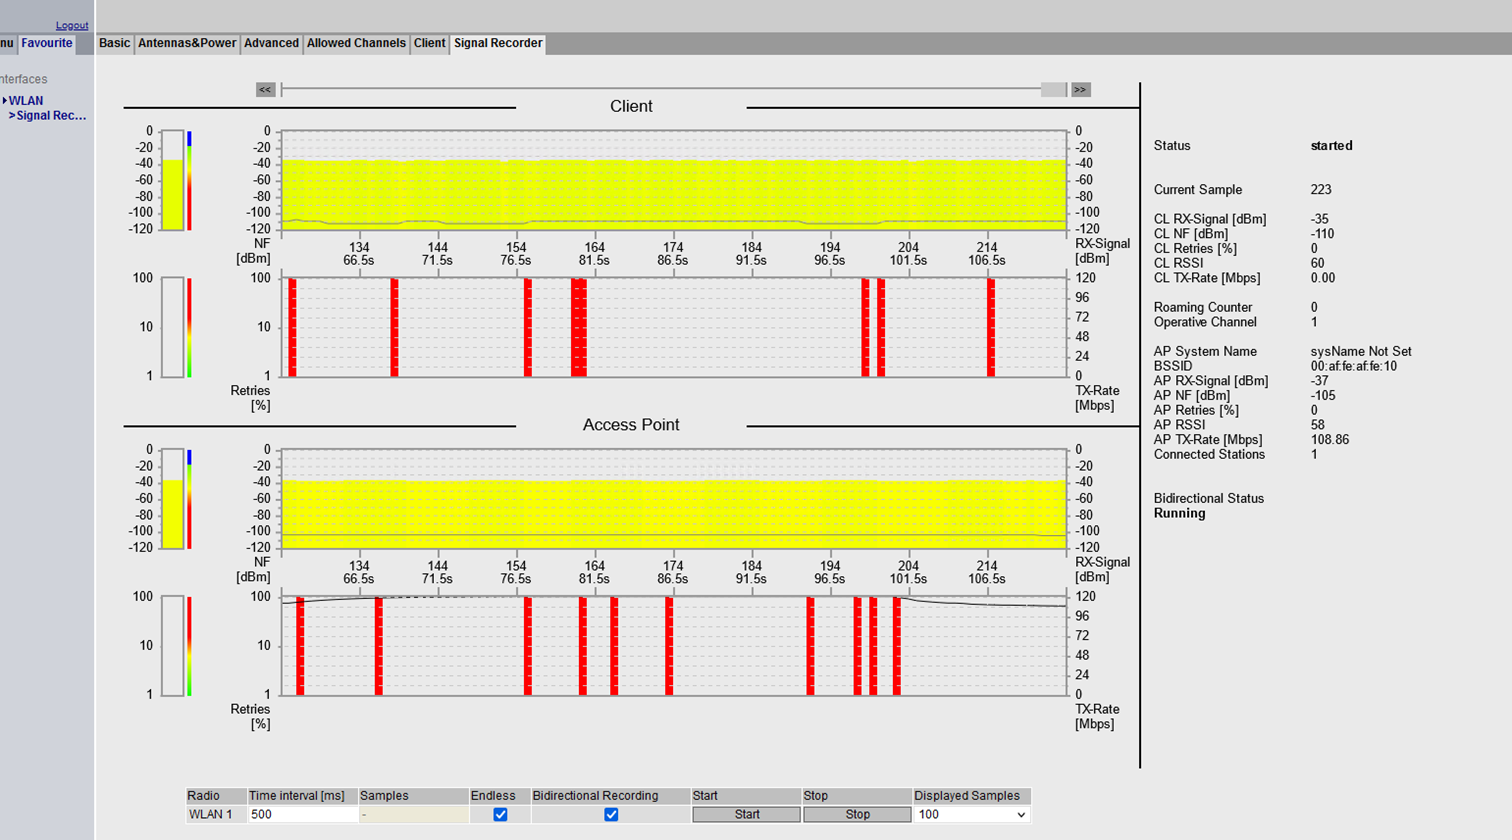
\includegraphics[width=\textwidth]{Pictures/Signalrecorder.png}
        \caption{Signalrecorder}
        \label{Signalrecorder}    
\end{figure}

\subsection{Recherche möglicher Lösungen - Ergebnisse}
\subsubsection{JavaScript embedded?}
\subsubsection{WebAssembly - Was ist das?}
Webassembly ist ein vom W3C festgelegter Standard, der einen Bytecode definiert, der in Webbrowsern aber auch außerhalb ausgeführt werden kann. \\
Die Version 1.0 wurde im März 2017 veröffentlicht und wird seitdem von allen gängigen Browser Engines unterstützt. \\
Unterstützt wird Webassembly in Chrome seit Chrome 57, in Firefox seit Firefox 52, in Edge seit Edge 16 und in Safari seit Safari 11. \cite*{caniusewasm} \\
\paragraph*{Vorteile}
\begin{itemize}
    \item   Multi Language Support - Webassembly unterstützt mehrere Sprachen. Es ist möglich WebAssembly als Kompilierziel für verschiedene Sprachen zu haben. \\
            Die Webassembly Entwickler unterstützen aktuell die Möglichkeit von C/C++ nach WebAssembly zu kompilieren. Des Weiteren gibt es einige kommerzielle und nicht kommerzielle
            Projekte, welche das Kompilieren von Rust, C\# und .NET, Ruby, Go, Java (sobald das Garbage Collection Proposal reif ist), PHP, Python, Haskell, Zig und Perl bereits ermöglichen.\\
            Die ermöglicht es Programmierern komplexe Funktionalität im Browser umzusetzen, ohne viel JavaScript zu nutzen. \\
            Außerdem ermöglicht es die Wiederverwendung von bereits bestehenden Implementationen.
    \item   Kompaktheit - Ein Webassembly File, welches die gleiche Funktionalität umsetzt wie ein JavaScript File kann bis zu 10 Mal kleiner sein und damit deutlich schneller bereitgestellt werden.
    \item   Portable - Webassembly ist sowohl zur Build-time als auch zur runtime von der Hardware unabhängig. Gebaut werden kann auf Windows, MacOS und Linux und die Webassembly PACKAGES
            können auf jedem Zielsystem ausgeführt werden, solange das Zielsystem die Webassembly Virtuelle Maschine unterstützt. Hier sei gesagt, dass zahlreiche Laufzeitumgebungen existieren, um 
            Webassembly auf einem diversen Feld verschiedener Hardwarearchitekturen lauffähig zu machen. 
    \item   Low Level Optimierungen - Das Webassembly Package kann mittels WAT (WebAssembly Text Format) dahingehend optimiert werden, dass die Low Level Instructions einzelner Funktioninen
            direkt manipulierbar und optimierbar sind. Dadruch ist eine größere Kontrolle über Ausführung, Performanz, Timing sowie die granulären Instruktionen möglich.
    \item   Bewährte Technologie(mit kleinen Abstrichen) - Sämtliche gängigen Browser unterstützen WebAssembly und es gibt schon einige beeindruckende und spannende Umsetzungen von Projekten in Webassembly
            welche bereits live eingesetzt werden und im Browser laufen. Als Beispiele für erfolgreiche Portierungen bzw. erfolgreiche Neuentwicklungen mit Webassembly dienen die Webapps von
            Adobe Photoshop sowie die Portierung des ComputerAidedDesign Tools AutoCAD der Firma Autodesk. Hier wurde WebAssembly genutzt um den hohen Leistungsbedarf sachgerecht im Browser abzubilden.
            Außerdem konnten sich die Firmen hier, insbesondere Autodesk, einen Teil der sonst nötigen Reimplementierung von Funktionalitäten sparen und den vorhandenen C bzw. C++ Code der Desktopversion
            von AutoCAD nutzen um die in C geschriebenen Programme mit deutlich geringerem Aufwand als einer Neuentwicklung in den Browser zu integrieren. Ein weiteres Produkt welches Webassembly
        	mit Erfolg eingesetzt hat und desses Lösung deutlich weniger performant gewesen wäre, ist das Entwurfswerkzeug für Benutzeroberflächen Figma. Hier wurde mittels C++ und React der hochperformante Teil der Funktionalität
            in WebAssembly implementiert.
    \item   Sicherheit - Die Webassembly virtuelle Maschine validiert WebAssembly Code bevor das Packet ausgeführt wird. Außerdem wird der Webassembly Code dann in einer speichersicheren Sandbox ausgeführt.
            Das bedeutet, dass Webassembly Code, welcher vom Internet abgerufen wird und im Browser ausgeführt wird von vorneherein stark beschränkt ist was den Zugang zu Hardware und Software
            Ressourcen auf dem ausführenden System angeht. Falls man den Code jedoch in einem Docker Container laufen lässt besteht die Möglichkeit vollen Netzwerkzugriff sowie den vollen Zugriff auf das Dateisystem zu nutzen.
\end{itemize}
\paragraph*{Nachteile}
\begin{itemize}
    \item   Aktuell sind noch keine eigenständigen Manipulationen der DOM verfügbar. Um komplexere Dinge zu ändern, muss das Webassembly → JavaScript Interface angesprochen werden
            und die DOM wird dann direkt von JavaScript manipuliert.
    \item   Aktuell maximal 4 Gibibytes Speicher adressierbar, es gibt ein Proposal, welches aktuell in Entwicklung ist, das zu beheben und dem
            Webassembly Module die Möglichkeit zu geben 32-Bit oder 64-Bit Speicher Indizes zu nutzen.
    \item   Der Anspruch JavaScript abzulösen, den das Projekt zu Anfang hatte, wird aktuell definitiv nicht erfüllt. Vor allem da beim aktuellen Stand sogenannter "Glue Code" in JavaScript benötigt 
            wird um das Webassembly Modul zu laden und vor allem um die Document Object Model (DOM) zu manipulieren.
\end{itemize}
\paragraph*{Analyse der Technologie}

\subsubsection{Tooling: Emscripten}
Emscripten ist ein Open-Source-Compiler-Tool, das C- und C++-Code in WebAssembly (WASM) und JavaScript konvertiert. Es wird derzeit von der Mozilla Foundation gepflegt. \\
WebAssembly ist wie bereits erwähnt ein neuerer Webstandard, der eine virtuelle Maschine für die Ausführung von kompiliertem Code im Webbrowser bereitstellt. Mit Emscripten können Entwickler vorhandenen C- oder C++-Code in WebAssembly-Code umwandeln, wodurch sie in der Lage sind, performante Anwendungen für das Web zu erstellen, die auf einer ähnlichen Geschwindigkeitsebene wie nativ kompilierte Anwendungen laufen können. \\
Der Compiler kann auch dazu verwendet werden, vorhandenen Code aus anderen Sprachen wie Rust, Fortran und anderen zu kompilieren. Die Ausgabe von Emscripten kann in verschiedenen Formaten erfolgen, wie zum Beispiel als reinem WebAssembly-Code oder als Kombination aus WebAssembly- und JavaScript-Code. Letzteres ist nützlich, wenn der Code auf älteren Browsern laufen muss, die noch keine vollständige WebAssembly-Unterstützung bieten. \\
Emscripten hat viele Anwendungsfälle, einschließlich der Erstellung von performanten Webanwendungen, die auf verschiedenen Geräten und Betriebssystemen laufen können, ohne dass dafür separate Anwendungen für jedes Betriebssystem erstellt werden müssen. Es kann auch für die Portierung von vorhandenem Code auf das Web verwendet werden, ohne dass der Code komplett neu geschrieben werden muss. Diese Eigenschaft wird ebenfalls in diesem Projekt genutzt. \\
Zusammengefasst ist Emscripten ein leistungsstarkes Werkzeug, das Entwicklern die Möglichkeit gibt, vorhandenen Code in das Web zu bringen und die Vorteile von WebAssembly zu nutzen, um performante Anwendungen im Browser auszuführen. Mit seiner flexiblen Ausgabeformatierung, seiner umfangreichen Bibliotheksunterstützung und seiner Unterstützung für Assembler-Code ist Emscripten eine wertvolle Ergänzung für jedes Entwicklungsprojekt, das darauf abzielt, performante Anwendungen im Web zu erstellen. \\
\cite*{emscriptenwebsite}
\subsubsection{Tooling: Bibliothek: SDL}
SDL (Simple DirectMedia Layer) ist eine plattformübergreifende Entwicklungsbibliothek, die Low-Level-Zugriff auf Audio-, Tastatur-, Maus-, Joystick- und Grafikhardware über OpenGL und Direct3D bietet. Sie wird von Entwicklern verwendet, um Videospiele, Multimedia-Software und andere Anwendungen zu erstellen, die Zugriff auf Multimedia-Hardware benötigen. \\
In diesem Projekt wurde die SDL Bibliothek genutzt, um zunächst primitive grafische Elemente zu erstellen, aus denen dann wiederum komplexere Anzeigeelemente erstellt wurden. Mit diesen komplexeren Elementen  ist es dann möglich sämtliche benötigten Darstellungen für den Signal Rekorder / System Rekorder in ausreichender Geschwindigkeit sowohl in jedem  unterstützten Webbrowser als auch nativ auf dem Gerät zu rendern. Die STL Bibliothek übersetzt allgemeine Grafikfunktionen je nach Kompilierziel in spezifische, der Hardware angepasste System Calls und fungiert somit als Abstraktionslayer. 
\cite*{sdlwebsite} \\
\subsection{Durchführung}
\subsubsection{Aufbau des Buildsystems}
Für die Validierung der Idee musste zunächst die Buildtoolchain der Emscripten Umgebung heruntergeladen und konfiguriert werden. 


\paragraph*{Buildsystem in Windows}
Der aktuell einfachste Weg ist, ein Repository von der Emscripten Foundation lokal auf den Rechner zu klonen und dann mit den im Ordner verfügbaren Skripten die Toolchain für die aktuelle Hardware aufzubauen. 
Im Anschluss muss dann die korrekte Funktionalität der Tool-Chain geprüft werden. Dies geschieht mit einer automatisierten Testsuite, welche diverse C-Skripte enthält, welche von der Tool Chain mit dem Ziel Webbrowser ( Ziel: Webassembly, Javascript Gluecode Und HTML) kompiliert werden und im Anschluss automatisiert getestet.
in der Testsuite findet man diverse Beispiele anhand derer man sich die Grundfunktionalität von Skripten herleiten kann und für die eigene Arbeit aus den einfachen Funktionsbeispielen komplexere Funktionalitäten aufbauen kann. \cite*{emscriptendownload}\\
\paragraph*{Buildsystem unter Linux}
Unter Linux ist der Aufbau des Buildsystems recht ähnlich. Unter Umständen muss man jedoch noch nötige Abhängigkeiten des Buildsystems über den paketmanager der Wahl installieren. \\

\paragraph*{Einbinden in die vorhandene Buildumgebung}
Dies wurde dann auch im Linux Build-system des Projekts getan und das Kompilieren von Skripten mit einem einfachen Beispielcode innerhalb des normalen Bauzyklus der Firmware geprüft. Dies war nach einigem Testen auch erfolgreich.
\subsection{Gewünschte Funktionen}
Für den Signalrecorder wurden im Vorhinein folgende Funktionalitäten vereinbart: \\
\begin{enumerate}
        \item Die korrekte Anzeige der am Endgerät von der jeweiligen Engine ausgegebenen Signalstärke ()\q{RX-Rate} Punkt diese sollte zusätzlich noch farblich codiert werden und für einen von mehreren wählbaren Zeitabständen auslesbar sein.
        \item Der sogenannte \q{noisefloor},  gemessen und berechnet von der jeweiligen engine, sollte im selben Graph für jeden Messpunkt als leicht verständlicher Linienverlauf dargestellt werden.
        \item Für die WLAN-Geräte sollte die Anzahl der \q{Retries}, das heißt der wiederholten Versuche den selben WLAN Frame zu senden, in Prozent von 0 \% bis 100 \% angezeigt werden. Dies kann zur Einschätzung von Störsignalen im Übertragungsmedium dienen.
        \item Die sogenannte TX-Rate des Endgeräts soll außerdem angezeigt werden,
        \item Für den bidirektionalen Betrieb sollen eben diese Kenngrößen, welche nach Anfrage vom Access Point mit übertragen werden  ebenso grafisch dargestellt werden.Dies ermöglicht den Vergleich der gesendeten und empfangenen kennzahlen eine Verbindung da die Parameter von Sender und Empfänger jeweils zeitgleich zur Verfügung stehen und damit analysiert werden können.  Dies ist vor allem für Mitarbeiter aus dem Support, für die Inbetriebnahme beim Kunden vor Ort oder auch für kundiges Personal beim Kunden hilfreich.
        \item Die polling rate, das heißt die Zeitintervalle nach denen jeweils ein neuer Daten bzw Messpunkt aufgezeichnet und dargestellt wird soll in Millisekunden in einem vorgegebenen Intervall frei wählbar sein.
        \item Die Anzahl der aufgenommenen Daten beziehungsweise Messpunkte soll von 100 bis 20000  definierbar sein. wahlweise soll auch ein zeitlich nicht begrenzter, das heißt endloser Betrieb des Signalrecorders möglich sein.
        \item Zusätzlich zur visuellen Darstellung der einzelnen Datenpunkte soll im Browser Modus des Signalrecorders der aktuell gemessene Datenpunkt mit allen vorhandenen Informationen, wie zum Beispiel die oben genannten signalparameter als auch beispielsweise der verwendete Channel, der Systemname des Accesspoints  oder die Anzahl der verbundenen WLAN Clients mit diesem Access Point.
        \item  Für den Wireless-Lan Fall:  bei einem sogenannten Roaming event, das heißt wenn bei sich überlappenden WLAN-Netzwerken der WLAN client in Bewegung ist oder sich die Sendeleistungen der Access Points verändern oder sich die Topographie der Umgebung so verändert dass die Empfangsleistung am Client für die verschiedenen Netzwerke sich über die Zeit ändert, dann  können moderne WLAN Clients, welche dieses Feature unterstützen, im Idealfall nahtlos von Netzwerk B zu Netzwerk B wechseln ohne dass es zu einer merklichen Unterbrechung der Datenübertragung kommt. diese Roaming Events sollten ebenfalls angezeigt werden wobei der  \q{Service Set Identifier}  des Netzwerks zu dem gewechselt wurde ebenfalls in der laufenden Grafik angezeigt wird Punkt so ist es sichtlich welche Datenpunkte zu dem neuen Access Point gehören.
        \item Des Weiteren sollte es möglich sein die Anzahl der angezeigten Datenpunkte aus einer vorgegebenen Menge an Auswahlmöglichkeiten dynamisch zu wählen.
        \item In einer Besprechung mit den verschiedenen Stakeholdern des Projekts wurden noch weitere  mögliche Zusatzfunktionen für den Signalrecorder definiert: 
                \begin{enumerate}
                        \item  Das Auslesen der gerätespezifischen Temperatursensoren und die  grafische Anzeige und Darstellung dieser Temperaturmessdaten, eventuell auch mit einer grafischen Repräsentation des sicheren Betriebsbereichs des jeweiligen Gerätes.
                        \item Das Auslesen von gerätespezifischen  Auslastungskennzahlen wie zum Beispiel,  der verfügbare freie Speicher oder die Auslastung der einzelnen Prozessorkerne beziehungsweise des Gesamtsystems.
                        \item Eine grafische Darstellung des sogenannten Netzwerk throughput. Dies ist eine Kennzahl welche die Rate derDaten Übermittlung in einem Netzwerk beschreibt. 
                        \item Die Anzeige sollte für verschiedene Nutzergruppen unterschiedlich auslegbar sein.
                        \item Alarme für diverse Events, eventuell beim Unterschreiten oder Überschreiten eines definierten Grenzwertes.
                        \item Eine spezielle Anzeige für den Siemens Support, welche weitere Kennzahlen anzeigen kann, zum Beispiel die Anzahl der Chip Resets seit Fertigung.
                        \item Der aktuelle/aggregierte Energieverbrauch
                        \item weitere spezifische Werte, unter anderem für Siemens spezifische Features der Geräte - zensiert aus Freigabegründen
                        \item Eine Möglichkeit den Signalrecorder automatisiert zu starten.
                        \item Eine graphische Kanalübersicht, sowohl bei Wireless-LAN Geräten als auch bei Mobilfunkgeräten, hier dann eine Bandübersicht.
                \end{enumerate}
\end{enumerate}
\subsection{Interaktion mit Legacy Code}
Da im Projekt bereits einige Vorarbeit für den Signalrecorder geleistet war, es gab bereits eine rudimentäre Version und Implementierung, welche jedoch allein im Wireless LAN Gerät genutzt werden konnte.  Im Zuge der Bearbeitung des Projektes  habe ich mich dann in den schon vorhandenen Programmcode eingearbeitet Punkt es gab ein in C geschriebenes Modul,  welches die Generierung einer PDF-Datei mit sämtlichen aufgenommenen Datenpunkten im Textformat sowie einer grafischen Darstellung einige dieser Punkte durchführte. \\
 Des Weiteren gab es eine Implementierung der Echtzeit Ansicht des signalrecorders im Webbrowser. Diese war geschrieben in JavaScript.  Hier funktioniert der Ablauf  folgendermaßen:
\begin{enumerate}
        \item Der Signalrecorder wird auf einem von mehreren möglichen Wegen gestartet und das Gerät stellt über eine vorher definierte URL die Datenpunkte, die zuletzt generiert wurden, seit dem letzten Abrufen der URL, in einem leicht verarbeitbaren Textformat zur Verfügung. dieser Text wird im Browser HTTP Fetch Request vom Gerät abgeholt.  der dabei entstehende String wird in mehreren Schritten dahingehend  verarbeitet, dass die einzelnen Datenpunkte mit einer kurzen Zugriffszeit im Speicher liegen und damit im Anschluss für die Generierung der grafischen Oberfläche verwendet werden können. \\
        \item Im Anschluss werden dann zunächst die eingestellten Anzeige Parameter, wie z.B die Anzahl der anzuzeigenden Datenpunkte,die Aktualisierungsgeschwindigkeit, die Laufzeit des Signalrecorders, als auch der verwendete Modus (bidirektionaler Modus oder nicht) verarbeitet und die Anzeige dementsprechend angepasst. Nun wird über  eine quasi endlos laufende Schleife für jeden Datenpunkt die Anzeige aktualisiert und der neue Datenpunkt wird grafisch dargestellt. Zeitgleich aktualisiert sich auch die textliche Beschreibung des aktuellen Datenpunktes. \\
        \item Nachdem der Signal Recorder entweder seinen vorher definierten laufzeitraum erreicht hat oder er von Hand über einen von mehreren Wegen, per Klick im web based management oder per direktem Kommando Zeilen Befehl ans Gerät, beendet wurde stellt das Gerät die aufgenommenen Daten über ein Download Menü sowohl in der generierten PDF Version als auch in der leichte zu verarbeitenden CSV Version zum Herunterladen zur Verfügung. \\
        \item Im Anschluss wird das gesamte Gerät wieder in einen Zustand gebracht, so dass neuerliches Aufnehmen von Daten möglich ist  uns sämtliche Einstellungen werden intern zurückgesetzt. \\
\end{enumerate}
Um möglichst schnell einen funktionierenden Prototypen zu generieren habe ich zunächst lediglich die Generierung der grafischen Oberfläche ausgelagert und die Datenverarbeitung der vom Gerät kommenden Daten im Großteil vom alten Javascript Code übernommen. Ich musste jedoch einige kleinere Änderungen vornehmen, da das Zusammenspiel zwischen dem reservierten webassembly-speicher und dem gewöhnlichen Speicher auf den der Javascript Code zugreift nicht trivial ist und hier einige Datenstrukturen angepasst werden mussten.  Problematisch war hier hauptsächlich dass Javascript kein typing kennt,  das heißt jede Variable kann jeden beliebigen Datentyp fassen und es ist zur Laufzeit nicht gewährleistet dass der Inhalt einer Variable eine definierte Länge im Speicher hat. 
Webassembly kann jedoch nur  mit wenigen primären Datentypen Umgehen. Die vorhandenen Datentypen sind: \\
\begin{enumerate}
        \item i32 : 32-bit integer
        \item i64 : 64-bit integer
        \item f32 : 32-bit floating point
        \item f64 : 64-bit floating point
\end{enumerate}
\begin{verbatim*}

\end{verbatim*}
Hier habe ich einige Zeit damit verbracht mir ein System zu überlegen wie ich die Daten aus dem JavaScript Speicher  ohne viele Rechenoperationen in passende webassembly bzw C-kompatible Datentypen umwandeln kann. Leider habe ich hier keine zufriedenstellende Lösung erzielen können und um mit dem Projekt voranzukommen habe ich dann einen anderen Weg eingeschlagen.  Statt der Datengenerierung  in JavaScript sollte lediglich das Webassembly-Modul durch JavaScript aufgerufen werden und die Abfrage der URL mit den aktuellen Daten Punkten sollte auch mittels C-Code realisiert werden. \\

\subsection{Wesentlicher Code}
\subsubsection{Grafikdarstellung mittels SDL}
Wie bereits weiter oben erwähnt erfolgt die  grafische Darstellung bzw. die Grafikgenerierung über Funktionalitäten, welche mit der SDL Bibliothek realisiert werden.
Hier ist es zunächst wichtig zu verstehen, wie diese Bibliothek arbeitet. \\
Grundsätzlich gibt es zwei verschiedene Arten, um auf einem Computersystem grafische Anzeigen zu realisieren. Zum einen kann für die Berechnung der Grafiken der Prozessor (CPU)  genutzt werden, alternativ dazu kann auch eine speziell dafür ausgelegte Hardware wie z.B eine Grafikkarte mit einem Grafikprozessor für die Berechnung der grafischen Inhalte verwendet werden.  Je nach Systemaufbau und Hardware-Bestückung ergeben sich hier natürlich Unterschiede. Im Allgemeinen kann jedoch als grobe Regel festgehalten werden, dass die Grafikberechnung über den Hauptprozessor langsam ist während die Grafikgenerierung über den Grafikprozessor eine höhere Geschwindigkeit aufweist. \\
Das liegt unter anderem daran, dass die CPU Probleme hat, sogenannte Texturen zu verarbeiten, während der Grafikprozessor mit seinen Instruktionen speziell darauf ausgelegt ist.  Wenn man keinen dedizierten Grafikprozessor hat, bleibt einem nur die Möglichkeit, die Grafiken  statt in Texturen in sogenannten  Oberflächen (Surfaces)  zu speichern und vom Computer darstellen zu lassen. \\
Die SDL Bibliothek steht hierbei als Abstraktionsmethode zwischen der Hardware und der Software und bietet die Möglichkeit allgemein mit der Nutzung von Texturen zu programmieren und je nach verfügbarer Hardware werden die notwendigen Systemaufrufe dann so umgesetzt dass die vorhandene Hardware optimal ausgenutzt wird.
\paragraph*{Erstellen eines Farbverlaufs}
Zunächst musste ein Weg gefunden werden, um die verschiedenen Signalparameter farblich so zu codieren, dass auf einen Blick ein Überblick über den aktuellen Zustand der Verbindung geschaffen werden kann. Zu diesem Zweck habe ich eine Funktion geschrieben, welche abhängig von für die Signalparameter passenden Grenzschwellen einen Farbverlauf generiert. Die Funktion sieht man hier, für die Farbgebung der Signalstärke: \\
\begin{lstlisting}[caption={Codeausschnitt - Generierung von Farbgradienten},captionpos=b,language=C]
        int createSdlColorsWithRGBMode(int mode){
                if (mode == MODE_DBM){
                    int red = 120;
                    int yellow = 40;
                    int blue = 15;
                    float tmp;
    
                    for (int i = 0; i<red;i++){
                        //0-15
                        if (i < blue){
                            colors[i].r = 0;
                            colors[i].g = 0;
                            colors[i].b = 255;
                            colors[i].a = 255;
                        }//15-40
                        else if(i < yellow){
                            tmp = (i-15)*10.2;
                            if (tmp < 10){
                                tmp = 0;
                            }else if(tmp>255){
                                tmp = 255;
                            }
                            colors[i].r = (int)tmp;
                            colors[i].g = 255;
                            colors[i].b = 0;
                            colors[i].a = 255;           
                        }//40-120
                        else if(i < red){
                            tmp = (i-40)*3.1875;
                            if (tmp < 3){
                                tmp = 0;
                            }else if(tmp>255){
                                tmp = 255;
                            }
                            colors[i].r = 255;
                            colors[i].g = 255-(int)tmp;
                            colors[i].b = 0;
                            colors[i].a = 255;            
                        }   
                    }
\end{lstlisting}
Die Funktionsweise ist leicht ersichtlich, jeder Wert zwischen 0 und -15 dBm ist Blau, das signalisiert eine optimale Signalstärke für WLAN. Ab -15 dBm bis -40 dBm, ist ein Farbverlauf, der von komplett Gelb über Orange langsam Rot wird und ab -40 dBm nahtlos in einen Farbverlauf übergeht bei dem nach und nach der Gelbanteil komplett verschwindet. 
\paragraph*{Säuberung der Zeichendaten}
Die Daten waren für die Darstellung auch noch zu säubern, was ich mit folgender Funktion realisiert habe:
\begin{lstlisting}[caption={Codeausschnitt - Säuberung des Arrays mit den Datenpunkten die für einen Frame gezeichnet werden},captionpos=b,language=C,breaklines]
int get_data_for_plotting_cl_dbm(datapoint buffer[NO_Of_DRAWPOINTS], int index){ //function to wrap data generation for plotting cl_db 
    #ifdef native //!< defined when compiling to run on Device
        for(int i=0;i<index+1;i++){
        read_data_from_csv("data/signal_recorder_wlan1.csv",buffer,index); //!< Read in the Data up until specified point
        }
    #endif
    #ifdef __EMSCRIPTEN__ //!<defined when compiling via emscripten to wasm, used in Browser
        for(int i=0;i < NO_Of_DRAWPOINTS;i++){          
            if (currentsample < NO_Of_DRAWPOINTS && i > (((currentsample - 1) % NO_OF_DATAPOINTS))){ //Case needed because garbage data is read before the array of datapoints actually begins.
                buffer[(NO_Of_DRAWPOINTS-1)-i].cl_rx_dbm = -1;//!< set to invalid value so nothing gets drawn
                buffer[(NO_Of_DRAWPOINTS-1)-i].cl_retry = 0;
                buffer[(NO_Of_DRAWPOINTS-1)-i].sample = 0;//set to zero so nothing gets drawn
                continue;
            }
            if(currentsample/NO_OF_DATAPOINTS > 0){//!<Case True Samplenumber>NO_OF_DATAPOINTS, prevent overflow of Dataarray
                if (i < currentsample%NO_OF_DATAPOINTS){//Case needed if some of the data is at then end of the Dataarray and some at the start because of Ringbuffer.
                    buffer[(NO_Of_DRAWPOINTS-1)-i] = alldata[(((currentsample-1) % NO_OF_DATAPOINTS))-i]; //
                    continue;
                };
                buffer[(NO_Of_DRAWPOINTS-1)-i] = alldata[((currentsample % NO_OF_DATAPOINTS)-i)+(NO_OF_DATAPOINTS-1)]; //
                continue;
            }            
            buffer[(NO_Of_DRAWPOINTS-1)-i] = alldata[(((currentsample - 1)% NO_OF_DATAPOINTS))-i]; //!< if no overflow at ring buffer just copy normaly
        }
    #endif
    return SUCCESS;
} 
\end{lstlisting}
Da für den Endlosbetrieb als Datenstruktur ein Ringbuffer genutzt wurde, ist es von nöten vor jedem zeichnen die Daten in einem speziellen Array abzuspeichern, aus dem dann per Iteration einfach gelesen werden kann.
So muss beim Einschalten des Signalrecorder sicher gestellt werden, dass nur echte Datenpunkte graphisch umgesetzt werden und im Falle einer Überschreitung der maximalen Anzahl an Speicherbaren Datenpunkten die Daten aus dem Ringbuffer korrekt ausgelesen werden und gegebenenfalls von der korrespondierenden Stelle am Ende des Buffers, der alle Daten enthält, ausgelesen und an der korrekten Stelle im Zeichenarray platziert werden. \\
%  DBM draw func
Mit den gesäuberten Daten muss jetzt noch die Höhe und Farbe der einzelnen Datenpunkte dargestellt werden. Hierfür wird die selbst geschriebene Funktion \q{draw\_column} genutzt. Sie ist im Grunde ein Abstraktionslayer um aus den primitiven Grafikobjekten in einer Zeile ein Rechteck mit definierten Startpunkten sowie einer einfach einzugebenden Farbe zu generieren. Die Folgende Funktion zeichnet dann für jeden Frame mit den Daten die passenden Rechtecke für alle anzuzeigenden Datenpunkte im kommenden Frame \\

\begin{lstlisting}[caption={Codeausschnitt - Zeichnen der Signalstärkekerzen},captionpos=b,language=C,breaklines]
int drawClientDBM(datapoint buffer[NO_Of_DRAWPOINTS], colorpalette dbmcolors,SDL_Surface * surface,SDL_Surface * realtimesurface){
    static int column_height, column_height_2;
    static double maxvalue = MAX_DBM;
    static double minvalue = MIN_DBM;
    static double maxpixel = CHART_HEIGHT;
    static double minpixel = 0; 
    static double m1 = (maxpixel-minpixel)/(maxvalue-minvalue); //calulate pixelheight dynamically
    //static double m2 = (minpixel-maxpixel)/(minvalue-maxvalue); //alternative function to calculate pixelheight

    for (int i=0;i<(NO_Of_DRAWPOINTS);i++){
        column_height = ((double)(-buffer[i].cl_rx_dbm))*m1 + (minpixel - m1 * minvalue) - minpixel;
        draw_column(surface,(i*COLUMN_WIDTH),column_height,COLUMN_WIDTH,(int)minpixel,0, dbmcolors.giveColor(buffer[i].cl_rx_dbm));
        if (i==(NO_Of_DRAWPOINTS-1)){ //draw most recent data with realtime column to realtime surface
            draw_column(realtimesurface,10,column_height,3*COLUMN_WIDTH,(int)minpixel,0, dbmcolors.giveColor(buffer[i].cl_rx_dbm));     
        }
    }
    return SUCCESS;
}
\end{lstlisting}
Zusätzlich zu der Anzeige von farbigen Objekten und Linien war es auch noch nötig Text zu rendern. Da die SDL Bibiliothek selbst sehr rudimentär ist unterstützt sie von Haus aus nicht das Rendern von Text. Es gibt aber eine Erweiterung der Bibliothek, genannt \q{SDL\_ttf}. Hiermit ist es möglich mit Strings Texturen und Surfaces zu erstellen, welche man dann mittels der SDL Bibliothek und einer Technik welche im Grafikrenderingbereich \q{blitting} genannt wird zusammenführen. Hier sind spezielle Vorraussetzungen zu erfüllen, da nicht jede Surface mit jeder anderen zusammengeführt werden kann. Teilweise müssen für das richtige Zusammenführen der Surfaces die Werte der einzelnen Pixel mit mathematischen Operationen überlagert werden, sodass man hier ein sinnvolles Ergebniss bekommt. \\
Jetzt wird noch auf eine Beispielfunktion eingegangen, anhand derer man die Funktion \q{Textrendering} sehen kann.
\begin{lstlisting}[caption={Codeausschnitt - Rendern von Text},captionpos=b,language=C,breaklines]
int draw_samplenumbers(SDL_Rect renderTarget,datapoint buffer[NO_Of_DRAWPOINTS] ,SDL_Surface *surface_of_Viewport){
        static char samplenumbers[NO_Of_DRAWPOINTS][MAX_LENGTH_SAMPLENUMBER];
        //get number of valid drawn samples
        for (int i = NO_Of_DRAWPOINTS - 1; i >= 0; i--)
        {
                if(buffer[i].sample != 0){ //check if empty data
                if (buffer[i].sample >99999 || buffer[i].sample < 1){
                        printf("Error in samplenumber length at i: %d and with: %d" , i, buffer[i].sample);
                        return FAILURE;
                        continue;
                }
                sprintf(samplenumbers[i],"%d",buffer[i].sample);
                continue;
                }
                sprintf(samplenumbers[i],"0");
        }
        SDL_Surface * bigSurfaceforSamplenumbers = SDL_CreateRGBSurfaceWithFormat(0,renderTarget.w,renderTarget.h,32,SDL_PIXELFORMAT_RGBA32);;
        SDL_Color writecolor = {30,0,0,255}; //create color for text
        SDL_Rect blitrect = {0,0,15,16}; //rectangle to define blit coordinates
        Maincontext.font_dbm = TTF_OpenFont(FONTPATH_EMSCRIPTEN, 12); //open font to render text
        #ifdef SAMPLENUMBER_IN_CHART_WANTED
        for (int i = 0; i < NO_Of_DRAWPOINTS; i++)
        {
            if (i%5 == 0) {//Only draw every 5th Samplenumber, else display is crowded
                SDL_Surface *text_surface = TTF_RenderUTF8_Blended(Maincontext.font_dbm,samplenumbers[i], writecolor); //this creates small surface with text 
                //{Checks for Errors in Surface generation}
                blitrect.x = i*COLUMN_WIDTH + (text_surface->w/2);
                blitrect.y = CHART_HEIGHT - text_surface->h - 10;
                blitrect.w = text_surface->w;
                blitrect.h = text_surface->h;
                int blit_success =  SDL_BlitSurface(text_surface,NULL,surface_of_Viewport, &blitrect);
                if (!(blit_success == 0)){
                    printf( "Unable to blit surfaces together! SDL Error on i: %d: %s \n",i, SDL_GetError() );
                }
                SDL_FreeSurface(text_surface);  //always free surfaces after usage --> memory leak
            }
        }        
\end{lstlisting}
% func for text


%%%%%%%%%%%%%%%%%%%%%%%%%%%%%%%%%%%%%%%%%%%%%%%%%%%
\section{Dauertestanlage}
\subsection{Aufgabenstellung}
\subsubsection{Integrationstest - Was ist das?}
Ein Integrationstest ist ein bestimmter Vorgang in der Softwareentwicklung oder in der Firmware Entwicklung wie jetzt in dem vorliegenden Fall und dort wird in regelmäßigen Abständen die aktuellste Änderung der Programmfunktionalität geprüft und ob durch die Änderungen bestehende Funktionalitäten gestört werden.  \\ 
Dazu wird in regelmäßigen Abständen, häufig sogenannte Nightly Builds,  ein bestimmter stand des Programmcodes und dessen Funktionalität kompiliert und automatisiert getestet. \\ 
Bei diesen Tests wird im Gegensatz zum Systemtest nicht die komplette Programmfunktionalität mit allen Eventualitäten geprüft sondern lediglich die Grundfunktionalität der einzelnen Features verifiziert und automatisiert ein Bericht erstellt. hierdurch können neue eingefügte Fehler in der Programmierung, sogenannte Bugs, zeitnah gefunden werden und bevor die Fehlersuche zu aufwendig und unübersichtlich wird diese Fehler behoben werden. man prüft hier nicht die vollständige Funktionalität ab weil das ab einer bestimmten Produktgröße schlicht nicht möglich ist. der so entstandene Bericht wird im Team be- und verarbeitet und am Ende des nächsten Arbeitstages werden die eingecheckten Änderungen am Programmcode erneut automatisiert überprüft.
 \\ Es gibt verschiedene Vorteile von Integrationstests. Zum einen können sie dazu beitragen, Probleme frühzeitig im Entwicklungsprozess zu erkennen und zu beheben. Wenn ein Problem während eines Integrationstests auftritt, kann es in der Regel einfacher behoben werden, da die Ursache des Problems schnell identifiziert werden kann.
\\
Ein weiterer Vorteil von Integrationstests besteht darin, dass sie dazu beitragen können, die Qualität des Produkts insgesamt zu verbessern. Durch das Testen der verschiedenen Komponenten einer Anwendung wird sichergestellt, dass sie korrekt funktionieren und dass alle Probleme behoben werden, bevor das Produkt an Kunden ausgeliefert wird.
\\
Zu meinem Eintritt in der Abteilung gab es drei  integrationstestanlagen für die verschiedenen Mobilgeräte, sowie drei Testanlagen für die industrial WLAN-Geräte.
 in diesem Testanlagen hängen diverse Geräte mit unterschiedlichen Funktionen beispielsweise Mobilfunkrouter der letzten sowie aktuellen Generation, DSL Router, so wie Ethernetrouter  welche auch Profinet unterstützen und als letztes Glied in der Nachrichtenkette vor der industriellen Anlage stehen.
 \\
 In diesen Integrationstestanlagen werden gezielt eng definierte Funktionen der Router auf  Hardware-Versionen getestet welche entweder nah bei oder auf dem Stand verkaufsfähiger Produkte sind.  \\
\\
Es gab schon einige vorhandene Testfälle sowie ein intern entwickeltes Tool, welches die Automatisierung und Auswertung der Testfälle vereinfacht ermöglicht. 
Wenn eine neue Funktionalität für eines der Produkte entwickelt wird, wird nach der ersten Fertigstellung eines Prototypen der Funktionalität ein neuer Testfall entwickelt und in die Integrations-Testanlage eingebaut.  \\
Hierzu wird zunächst genau abgesteckt, welches Ergebnis die Funktionalität haben soll, mit welchen Parametern gearbeitet wird, welche Zwischenzustände im Gerät notwendig sind, um die Funktionalität zu ermöglichen und schließlich wird eine technische Umsetzung all diese Voraussetzungen erstellt und geprüft. ist diese erste Test erfolgreich und ist man sich sicher, dass die zu prüfende Funktionalität auch tatsächlich geprüft wird, dann wird  der Test automatisiert und schlussendlich in die Anlage eingebaut. \\
Vor  allen  die Prüfung ob die gesuchte Funktionalität tatsächlich überprüft wird ist nicht immer trivial da beispielsweise im Netzwerk Kontext ausgeschlossen werden muss dass gesendete und empfangene Datenpakete über mögliche andere Wege z.B Internet oder Mobilfunkverbindung ihren Weg an das Ziel gefunden haben.\\
Beispiele für Testfälle sind das korrekte Wiederherstellen einer Mobilfunkverbindung nach dem Neustart des Gerätes, sei es durch Stromausfall, einen soft reboot durch den Benutzer ausgelöst, einen absichtlich produzierten Crash des Geräts, oder das Drücken der Reset-Taste. \\
\subsection{Bisheriger Stand}
Im Zuge der Verwendung  neuerer oder anderer Mobilfunk oder Wi-Fi engines müssen diese neuen Hardware Module auch getestet werden und es muss  durch Integrationstests sichergestellt werden sämtliche bereits implementierte Geräte Funktionalität auch auf der neuen Hardware lauffähig und performant ist.   \\
Da ständig neue Hardware-Versionen geprüft und getestet werden war es sinnvoll und notwendig eine  Dauertestanlage für eben solche Änderungen im Hardware Design  aufzubauen und in Betrieb zu nehmen. \\
Zufälligerweise gab es während meines Praxis Semesters eben eine solche Hardwareänderung und ich wurde zusammen mit einem Kollegen mit der Planung, der Beschaffung, dem Aufbau und der Inbetriebnahme sowie der Vernetzung mit der bestehenden Infrastruktur betraut. \\

\subsection{Durchführung}
Nach der Initialbesprechung zum Thema Dauertestanlage  haben wir intern im Team die Aufgaben verteilt und ich habe mich um die Stromversorgung sowie die Möglichkeit die Anlage remote, das heißt ohne örtlichen Zugang, bedienen zu können gekümmert.  Für den Aufbau konnten wir eine bereits vorhandene Hutschiene samt Käfig nutzen und es war nur noch nötig  die passenden Stromversorgungen zu besorgen, anzuschließen und im Anschluss zu verkabeln.  \\
Bei der Verkabelung war es wichtig und notwendig alle Geräte über einen externen ansprechbares Relais schalten zu können für welches ich ebenso die Verkabelung sowie Kaskadierung übernommen habe. Leider  ist eines der verwendeten Relais nicht funktionsfähig geliefert worden wodurch ich einige Zeit mit der Fehler Lokalisierung beschäftigt war. nachdem das kaputte Relais jedoch isoliert war und ein weiteres auf Lager war konnte dies schnell behoben werden und die Arbeiten konnten abgeschlossen werden \\
Für das Finden des Relais-Fehlers habe ich ein vom Hersteller bereitgestelltes Software Tool, welches die Funktionalität der Relais darstellen sollte, genutzt und konnte damit die seriellen Antwort und Acknowledgement Übertragungen Dahingehend auswerten die Fehler Lokalisierungen einfacher und schneller durchzuführen. Des Weiteren habe ich mich noch intensiv mit der Verwendung des seriellen Übertragungsprotokolls der Relais-Boxen auseinandergesetzt. \\
Im Anschluss habe ich mich noch um die Ethernet Verbindung der einzelnen Geräte untereinander sowie mit der Verbindung der gesamten Anlage mit der restlichen Infrastruktur und den nötigen Testcomputern beschäftigt.  \\

\subsection{Hardware}
Welche Hardware wurde hier verbaut und warum?
\begin{itemize}
        \item Relaisboard: \\
                Zur Fernsteuerung und im Falle einer Fehlfunktion verfügt die Anlage über die Möglichkeit den Strom zu einzelnen Geräten an und abzuschalten. Für die vorliegende Anlage wurden 3 Relaisboards kaskadiert, sodass nur ein einziger Anschluss an den Steuerungsrechner benötigt wird. \\
                Der Anschluss an den Steuerungsrechner erfolgt über eine serielle auf RS232 genormte Verbindung mit einem proprietären Protokoll für die Verbindung. Aufgrund von benötigter Fehlerfindungsarbeit war es nötig, dass ich mich genauer mit dem Protokoll beschäftigt habe um einen Übertragungsfehler zu lokalisieren. \\
                In der Testsoftware ist bereits eine Implementierung der Grundfunktionen des Protokolls implementiert, jedoch nicht genug für Debuggingzwecke.
        \item Steuercomputer: \\
                Für die Verwaltung der Anlage wurde ein Windows 10 Personal Computer mit ausreichender Anschlussmöglichkeit für sämtliche Geräte genutzt. \\
                Das Betriebssystem wurde gewählt, um den Verwaltungs- und Wartungsaufwand möglichst klein zu halten und eine gemeinsame Plattform mit allen anderen Anlagen zu haben. \\
                Außerdem ist das Testtool in seiner aktuellen Fassung nur auf einem Windows Betriebssystem lauffähig und dieses wird zwinged im Betrieb der Anlage benötigt.

        \item Administrierbare Layer 3 Switches: \\
                Für die Kommunikation über Ethernet-Verbindungen auf denen unter anderem auch der PROFINET Datenverkehr läuft, war es unabdinglich hier sogenannte \q{managed} Switches zu nutzen. \\
                Um den Anlagen Aufbau so kundennah und realistisch wie möglich zu halten wurden hierfür Hausprodukte mit ausreichender Portanzahl gewählt. Das besondere an \q{managed} Switches ist, dass sie die Möglichkeit bieten direkt in den Arbeitsprozess des Switches einzugreifen und beispielsweise selbst definierte Virtualle Lan Verbindungen, sogenannte VLAN's zu verwenden und so den Netzwerkverkehr abzugrenzen und zu Steuern. Des weiteren haben die speziell für diesen Anwendungszweck von Siemens hergestellten Switches zahlreiche zusätzliche Eigenschaften, die ihren Einsatz im Industrieumfeld begünstigen. 
        \item Einplatinenrechner: \\
                Für die Umsetzung von verschiedenen Testfällen und Anwendungszwecken wurden mehrere Einplatinenenrechner, hier ein Produkt von der Raspberry Pi Foundation. \\
                Als Beispiel für mögliche Testaufbauten mit den Einplatinenrechner dient die automatisierte Geschwindigkeitsmessung mit einer Performance Testing Suite. 
        \item Ethernetkabel \\
                Für die Netzwerkverkabelung wurden CAT6 Ethernet Kabel mit RJ45-Steckern genutzt. Besonders wichtig war hier, da auch die Geschwindigkeit und Qualität der Verbindung mit verschiedenen Endgeräten geprüft werden sollte, dass die Ethernetkabel keinen verschlechternden Einfluss auf die Geschwindigkeitsmessung haben. \\
        \item SCALANCE MUM 853-1 \\
        Der kompakte SCALANCE MUM853-1 Router ist für den Einsatz im Schaltschrank designt. Mit dem Gerät kann 5G in industriellen Anwendungen genutzt werden. Der eingebaute IPv6 Support und die Unterstützung vorheriger Mobilfunkstandards( 4G, 3G), wenn 5G Konnektivität nicht verfügbar ist machen das Gerät zu einem Innovativen Einsatzgerät in der industriellen Kommunikationsstrategie. \cite*{SCALANCEMUM} \\
        Zu sehen ist das Gerät in Abbildung \ref*{SCALANCEMUM}        
        \item SCALANCE S615 \\
        Mit den Industrial Security Appliances SCALANCE S, hier S615, lässt sich ein industrielles Netzwerk nahtlos an die Security-Strukturen der Office- und IT-Welt anschließen. Dabei erfüllen die Security Appliances die speziellen Anforderungen der Automatisierungstechnik, wie beispielsweise leichte Hochrüstbarkeit bestehender Anlagen, einfache Inbetriebnahme oder geringe Stillstandszeiten im Fehlerfall. \cite*{SCALANCES615}\\
        Hier in der Anlage wurde der S615 genutzt um die VXLAN Funktionalität zu testen.
\end{itemize}
\begin{figure}[!ht]
        \centering
        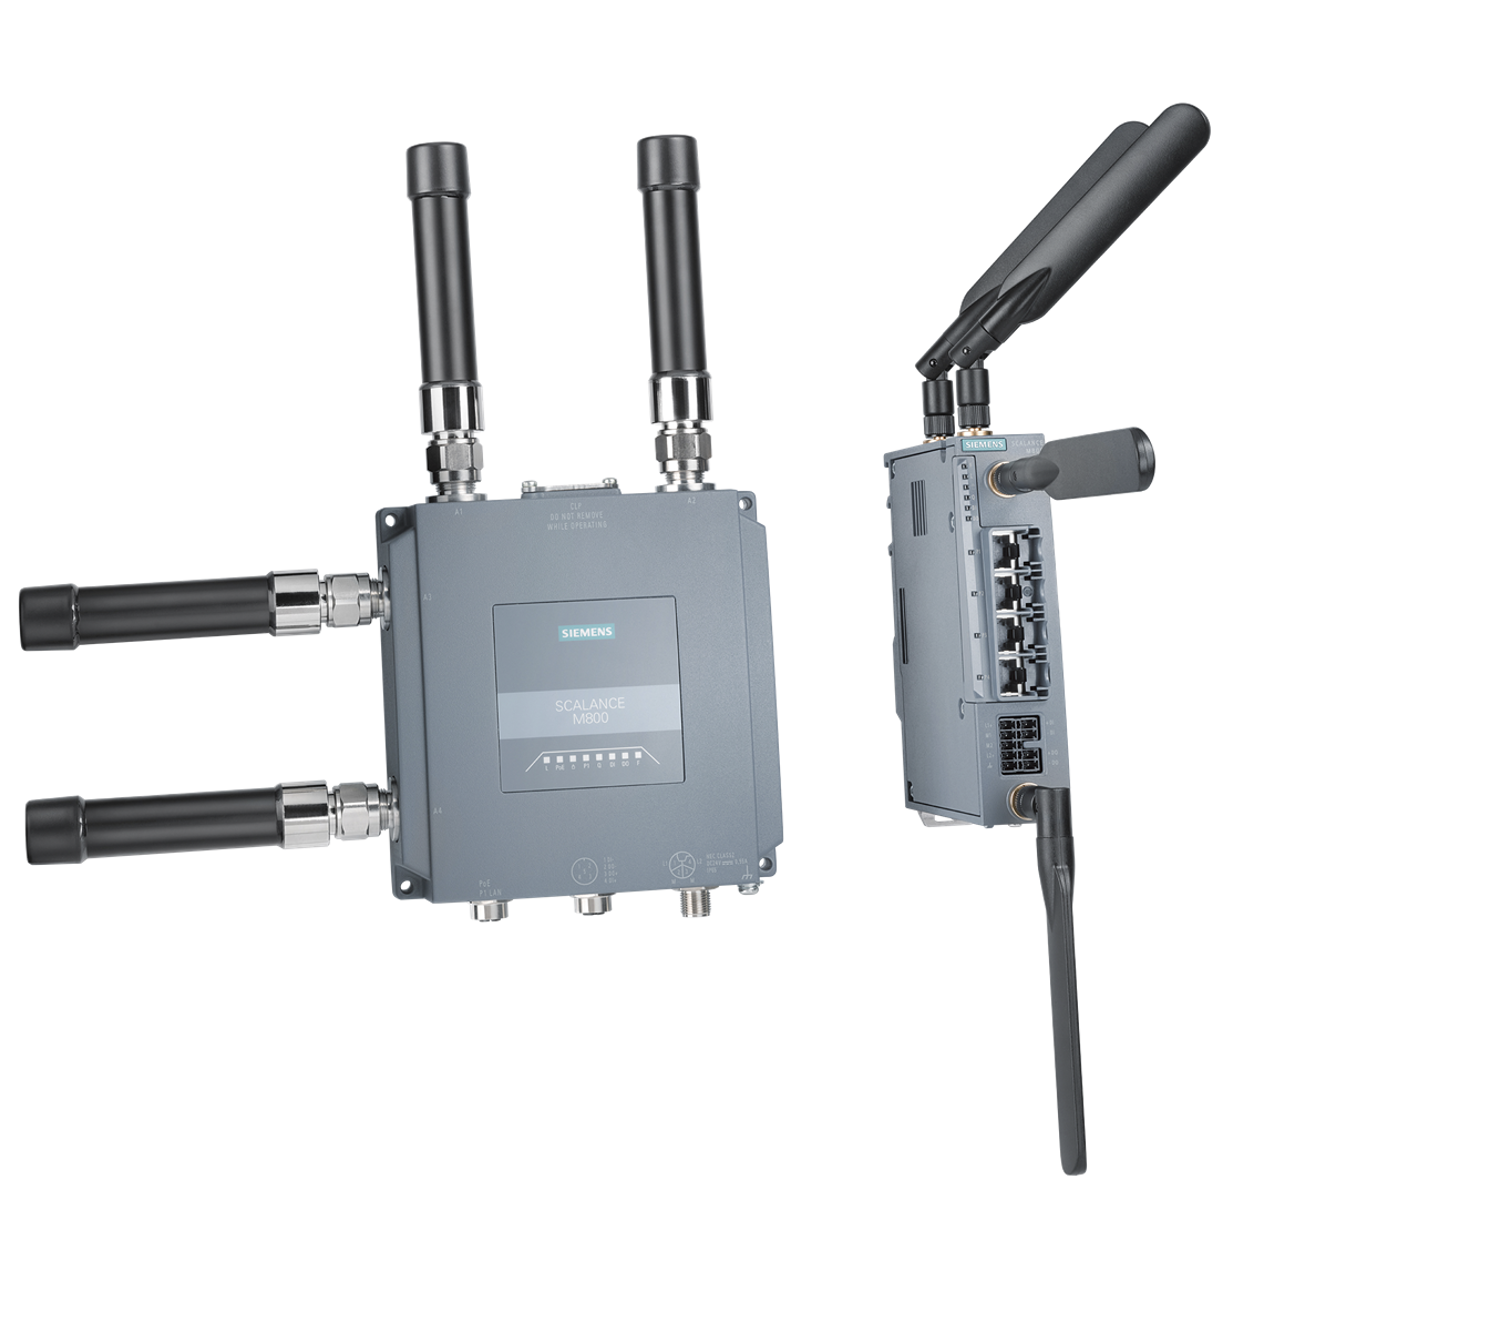
\includegraphics[width=\textwidth]{Pictures/MUM_IP65_IP30.png}
        \caption{SCALANCE MUM - 856-1(l) und 853-1(r)}
        \label{SCALANCEMUM}    
\end{figure}

\subsection{Software}
Für die Automatisierung der Dauertestanlage wurden verschiedene Softwarelösungen genutzt. \\
\begin{enumerate}
        \item  Das Intern entwickelte Automatisierungstool für Testfälle wurde für die Station eingerichtet und angepasst sowie an die Datenauswertungsinfrastruktur angeschlossen. Im Anschluss wurden kleinere Standard Testfälle durchgeführt und validiert dass die Anlage ordnungsgemäß arbeitet und die Ergebnisse ordnungsgemäß und richtig abgelegt und archiviert werden. \\
        \item  Für den reibungslosen Betrieb der Anlage mussten diverse Treiber und Software Tools auf dem Steuerungsrechner installiert werden. Unter anderem die Treiber  für die seriellen Schnittstellen, benötigte Software für Profinet Kommunikation und ein TFTP Server. \\
        \item  Auf den Einplatinencomputern mussten die Betriebssysteme neu installiert werden und im Anschluss daran sicherheitsrelevante Einstellungen getroffen werden. Nachdem dieses sowie die Netzwerkeinrichtung abgeschlossen war wurden noch weitere Software Tools installiert die für kommende Testzwecke  benötigt werden. \\
\end{enumerate}

% \subsection{Ergebniss}
% Die Testanlage läuft und kann für zukünftig notwendige Tests weiter ausgebaut oder umgebaut werden.
\section{Kleinere Projekte}
\subsection{Vorbereitung eines Kundenprojekts}
Im Zuge der Vorbereitung eines Kundenprojekts habe ich einen automatisierten Testaufbau für Geschwindigkeitstests an verschiedenen 5G-Netzwerken eingerichtet und den Test durchgeführt und ausgewertet.
\subsection{Pflegen der Testanlage}
Diverse kleinere Testfälle wurden von mir überarbeitet und die automatisierte Testanlage für die Integrationstest modifiziert.
\subsection{Testen von neuen GPS Features}
Für die Funktionsprüfung eines neuen Features im GPS Bereich habe ich Tests durchgeführt und zum Ende des Praktikums begonnen ein Tool zur weiteren Verarbeitung von GPS Daten zu schreiben.
